\documentclass[11pt,a4paper]{article}

% -----------------------------
% Essential Packages (foundations first)
% -----------------------------
\usepackage[utf8]{inputenc}
\usepackage[T1]{fontenc}
\usepackage{lmodern}
\usepackage[final]{microtype}

% Math
\usepackage{amsmath, amssymb}
\usepackage{mathtools}

% Graphics and figures
\usepackage{graphicx}
\usepackage{tikz}
\usetikzlibrary{positioning,arrows.meta,calc}
\usepackage{pgfplots}
\pgfplotsset{compat=1.18}

% Geometry
\usepackage[margin=2.5cm]{geometry}

% Tables and numbers
\usepackage{booktabs}
\usepackage{multirow}
\usepackage{siunitx}
\sisetup{
  round-mode=places,
  round-precision=2,
  table-number-alignment=center,
  detect-all,
}

% Floats and layout
\usepackage{float}
\usepackage[section]{placeins}
\usepackage{caption}
\usepackage{subcaption}

% Lists
\usepackage{enumitem}

% Citations (load before hyperref)
\usepackage[numbers,sort&compress]{natbib}

% URLs (improves line-breaking in links)
\usepackage{xurl}

% Hyperlinks (load late)
\usepackage[colorlinks=true,citecolor=blue,linkcolor=black,urlcolor=blue]{hyperref}
\Urlmuskip=0mu plus 1mu

% Clever references (load after hyperref)
\usepackage[capitalise,nameinlink]{cleveref}

% Counters and numbering
\usepackage{chngcntr}
\counterwithin{table}{section}
\counterwithin{figure}{section}

% Reduce overfull boxes
\emergencystretch=1em

% -----------------------------
% Custom commands
% -----------------------------
\newcommand{\methodfmt}[1]{%
  {\begingroup\catcode`\_=12\relax\texttt{#1}\endgroup}%
}

% -----------------------------
% Title and Authors
% -----------------------------
\title{On the Theory and Application of Singular Value Decomposition in Image Processing and Data Analysis}

\author{
  Gayane Ghazaryan\\
  \textit{Institute of Physics, Yerevan State University, Armenia}\\
  \texttt{gayane.ghazaryan@ysu.am}
  \and
  Artashes Ghazaryan\\
  \textit{Provectus Research; Technical University of Munich, Germany}\\
  \texttt{artashes.ghazaryan17@gmail.com}
}

\date{\today}



% -----------------------------
% Document
% -----------------------------
\begin{document}
\maketitle
\begin{abstract}
Singular Value Decomposition (SVD) is a fundamental factorization method central to image processing, dimensionality reduction, and numerical linear algebra. Its practical strength lies in truncating small singular values, thereby reducing storage while preserving the essential structure. The key challenge is choosing the truncation rank, which determines the trade-off between accuracy, efficiency, and stability.

We introduce an adaptive rank selection method that combines cumulative-energy thresholds with automated elbow detection, yielding a principled alternative to ad hoc rules. The framework is validated on image compression, denoising, and principal component analysis (PCA), with benchmarks against eigenvalue decomposition (EVD) and QR factorization. The results show that the adaptive rule improves fidelity and reproducibility, especially for noisy or ill-conditioned data.

All code, figures, and tables are released as open source, ensuring that the experiments can be reproduced in a clean environment. This unifies theory, automation, and reproducibility, reaffirming that SVD is both mathematically optimal and practically versatile for contemporary data analysis.
\end{abstract}

\paragraph{Keywords:}
Singular Value Decomposition; adaptive rank selection; cumulative energy; elbow detection; image denoising; image compression; principal component analysis.

% -----------------------------
% Main content
% -----------------------------

\section{Introduction}
\label{sec:intro}

Singular Value Decomposition (SVD) is a cornerstone of numerical linear algebra and a central tool in data science, machine learning, and image processing~\cite{golub2013matrix,hansen1987truncated,wall2003svd}. Its optimality for low-rank approximation, established by the Eckart--Young--Mirsky theorem~\cite{eckart1936approximation,golub2013matrix}, explains its broad use in image compression~\cite{andrews1976svd,swathi2017svd}, noise reduction~\cite{hansen2010discrete,guo2016svddenoise,gu2014wnnm,candes2011robust}, and dimensionality reduction via principal component analysis (PCA)~\cite{jolliffe2016pca,halko2011finding,lin2016lowrankreview}.  

Despite its elegance, a persistent practical difficulty is the choice of truncation rank $k$. This parameter determines the balance between fidelity, compression ratio, and computational cost~\cite{hansen1998rank,gavish2014optimal}. Existing strategies rely either on cumulative-energy thresholds, which require task-specific tuning, or elbow rules, which tend to underestimate the rank when singular values decay gradually~\cite{satopaa2011kneedle}. Consequently, applications often rely on ad hoc heuristics, which reduce reproducibility.

In this work, we propose an adaptive rank selection strategy that integrates cumulative energy and elbow detection within a unified SVD pipeline.
Concretely, we adopt a conservative hybrid rule
\[
k^\star = \max\!\bigl(k_\tau,\,k_{\text{elbow}}\bigr),
\]
which guards against under-selection while preserving interpretability.
Defaults such as $\tau\approx0.995$ are reliable for clean images. 
On standard images (e.g., \texttt{astronaut}, \texttt{cameraman}), the hybrid rule avoids elbow under-selection and maintains a higher structural similarity at comparable ranks (see \cref{sec:applications,fig:adaptive_vs_manual}).

\paragraph{Positioning vs.\ alternatives.}
Classical fixed-rank tuning lacks reproducibility. Energy thresholds are interpretable but require task-dependent choices of~$\tau$. 
Elbow rules adapt automatically but tend to under-select when the singular values decay slowly. 
Denoising-specific criteria such as optimal hard thresholding~\cite{gavish2014optimal} assume particular noise models 
and are not directly comparable across tasks, such as compression or PCA. 
In contrast, our hybrid rule is task-agnostic, reproducible, and guards against under-selection, without requiring prior calibration.

\paragraph{Contributions.}
The main contribution of this work is methodological and reproducibility-oriented.
\begin{itemize}[leftmargin=*,noitemsep,topsep=0pt]
  \item \textbf{Unified framework.} A reproducible SVD workflow for image compression, denoising, and PCA with standardized inputs and metrics (PSNR, SSIM, energy retention, and runtime).
  \item \textbf{Adaptive rank selection.} A principled hybrid of cumulative energy and elbow criteria, robust to slow spectral decay.
  \item \textbf{Systematic benchmarking.} Comparisons against EVD and QR factorization under identical conditions, clarifying the trade-offs in accuracy and runtime.
  \item \textbf{Open-source reproducibility.}
All Python scripts can regenerate every figure and table from a clean environment using fixed random seeds, explicit data sources, and version-pinned dependencies.

\end{itemize}

\textit{Scope and limitations.} We focus on standard truncated SVD for moderate-scale images and matrices; randomized or streaming variants are beyond the scope of this study.

\section{Mathematical Foundations of Singular Value Decomposition}
\label{sec:math-foundations}

\subsection{Definition and existence}
For any matrix \(A \in \mathbb{R}^{m \times n}\) with rank \(r \le \min(m,n)\), the \textbf{singular value decomposition (SVD)} is
\[
A \;=\; U \,\Sigma\, V^\top,
\]
where \(U \in \mathbb{R}^{m \times m}\) and \(V \in \mathbb{R}^{n \times n}\) are orthogonal, and
\(\Sigma \in \mathbb{R}^{m \times n}\) is diagonal (rectangular) with entries
\(\sigma_1 \ge \sigma_2 \ge \cdots \ge \sigma_r > 0\) on the main diagonal and zeros elsewhere. 
The SVD exists for every real (and complex) matrix, regardless of its shape or rank~\cite{golub2013matrix,trefethen1997numerical}. 
The singular values are unique; the singular vectors are unique up to orthogonal transformations within degenerate singular subspaces (e.g., sign flips or rotations when some \(\sigma_i\) coincide)~\cite{horn2012matrix}.\footnote{For complex matrices, orthogonal/unitary and transpose/conjugate-transpose are replaced accordingly.}

\subsection{Relation to eigendecomposition}
SVD is tied to the eigendecomposition of symmetric positive semidefinite matrices \(A^\top A\) and \(A A^\top\)~\cite{golub2013matrix,horn2012matrix}:
\begin{itemize}
    \item Columns of \(V\) are eigenvectors of \(A^\top A\) with eigenvalues \(\lambda_i = \sigma_i^2\);
    \item Columns of \(U\) are eigenvectors of \(A A^\top\) with the same nonzero eigenvalues;
    \item Hence \(\sigma_i = \sqrt{\lambda_i(A^\top A)}\).
\end{itemize}
Consequently, \(\{u_i\}\) and \(\{v_i\}\) form orthonormal bases for the column and row spaces of \(A\), respectively, and describe the directions of maximal variance/energy in the data representations.

\subsection{Optimal low-rank approximation}
Let \(A_k = \sum_{i=1}^{k} \sigma_i u_i v_i^\top\) be the rank-\(k\) truncation. 
The Eckart--Young--Mirsky theorem~\cite{eckart1936approximation,mirsky1960symmetric} states that \(A_k\) is the \emph{best} rank-\(k\) approximation to \(A\) in all unitarily invariant norms, in particular
\[
\|A - A_k\|_F \;=\; \min_{\mathrm{rank}(B)\le k} \|A-B\|_F \;=\; \Big(\sum_{i=k+1}^{r} \sigma_i^2\Big)^{\!1/2}, 
\qquad
\|A - A_k\|_2 \;=\; 
\begin{cases}
\sigma_{k+1}, & k < r,\\[2pt]
0, & k \ge r.
\end{cases}
\]
These identities justify the use of truncated SVD for compression, denoising, and dimensionality reduction.

\subsection{Compact and truncated forms}
Two reduced forms are especially useful~\cite{klema1980svd,golub2013matrix}:
\begin{itemize}
    \item \textbf{Compact (thin) SVD:} \(A = U_r \Sigma_r V_r^\top\), with \(U_r \in \mathbb{R}^{m \times r}\), \(\Sigma_r \in \mathbb{R}^{r \times r}\) (nonzero singular values), \(V_r \in \mathbb{R}^{n \times r}\). This is an exact factorization with minimal storage requirement.
    \item \textbf{Truncated SVD:} \(A_k = U_k \Sigma_k V_k^\top\) for \(k < r\), where \(U_k \in \mathbb{R}^{m \times k}\), \(\Sigma_k \in \mathbb{R}^{k \times k}\), \(V_k \in \mathbb{R}^{n \times k}\). This trades accuracy for efficiency by retaining the dominant components.
\end{itemize}
Two useful projection identities are
\[
A_k \;=\; U_k U_k^\top A \;=\; A V_k V_k^\top,
\]
showing that truncation amounts to an orthogonal projection onto the leading left/right singular subspaces.

\subsection{Energy, variance, and explained proportion}
\label{sec:energy}
SVD provides an orthogonally invariant notion of the total energy as follows:
\[
\|A\|_F^2 = \sum_{i=1}^{r} \sigma_i^2.
\]
For a rank-$k$ truncation $A_k$, the retained fraction is
\[
\eta_k \;\coloneqq\; \frac{\|A_k\|_F^2}{\|A\|_F^2} \;=\; \frac{\sum_{i=1}^{k} \sigma_i^2}{\sum_{i=1}^{r} \sigma_i^2}, 
\qquad k=1,\dots,r.
\]
This coincides with the explained variance in PCA for mean-centered data~\cite{jolliffe2016pca}. 
The quantity $\eta_k$ underlies the cumulative-energy thresholds used later for adaptive rank selection and provides a task-agnostic basis for comparing datasets.

\medskip
These properties establish SVD as both theoretically optimal and practically versatile. 
In the next section, we build on them to address the central challenge of choosing the truncation rank $k$, and propose an adaptive rule that avoids ad hoc heuristics.

\section{Adaptive Rank Selection}
\label{sec:adaptive}

Choosing the truncation rank \(k\) is the central practical challenge in applying SVD, as it sets the trade-off between the reconstruction fidelity, storage, and runtime. 
We propose a \textbf{unified adaptive rank selection} strategy that replaces ad hoc heuristics with principled and reproducible rules. 
The method combines two complementary criteria: a cumulative-energy threshold, which is standard in PCA practice~\cite{jolliffe2016pca}, and automated elbow detection via the Kneedle algorithm~\cite{satopaa2011kneedle}. 
Together, they yield stable choices for both sharply and slowly decaying singular spectra.

\subsection{Cumulative-energy criterion}
As introduced in \cref{sec:energy}, the cumulative-energy ratio $\eta_k$ measures the fraction of total energy retained by the first $k$ singular values. The threshold rule selects the smallest $k_\tau$ such that $\eta_{k_\tau}\ge\tau$, with $\tau\in(0,1)$. 
High thresholds (e.g., $\tau\approx0.995$) preserve fine details in compression, whereas lower values may be acceptable when noise dominates the tail. 
The sensitivity to $\tau$ is summarized in Appendix~\ref{sec:appendix-bench}.

\subsection{Elbow detection on the cumulative curve}
To improve robustness, we pair the threshold rule with elbow detection. 
We apply Kneedle~\cite{satopaa2011kneedle} to the \emph{cumulative} spectrum, using the normalized points \(\bigl(k/r,\,\eta_k\bigr)\) after light smoothing (Savitzky--Golay) to reduce jitter. 
Kneedle returns an elbow index \(k_e\) corresponding to the onset of diminishing returns in cumulative energy. 
Thus, we obtain two candidates: \(k_\tau\) from the threshold rule and \(k_e\) from the elbow detection.
We round the continuous elbow location to the nearest integer \(k\in\{1,\dots,r\}\).

\begin{figure}[t]
\centering
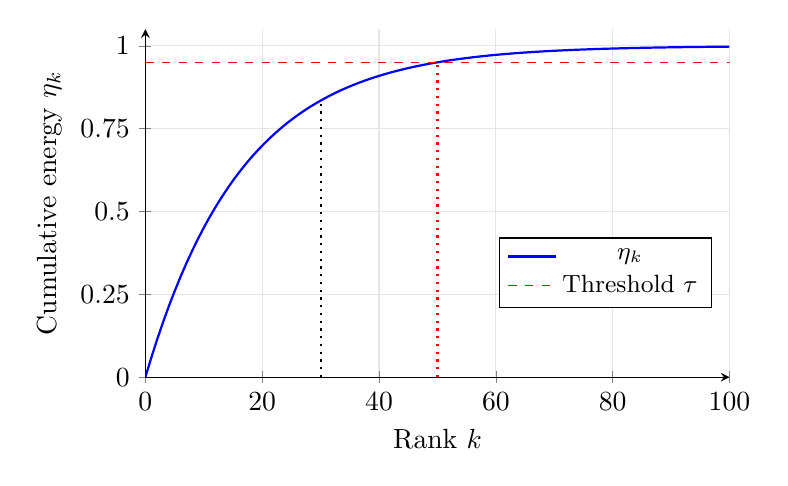
\begin{tikzpicture}
\begin{axis}[
    width=9cm, height=6cm,
    xlabel={Rank $k$}, ylabel={Cumulative energy $\eta_k$},
    xmin=0, xmax=100, ymin=0, ymax=1.05,
    grid=both, grid style={gray!20}, axis lines=left,
    xtick={0,20,40,60,80,100}, ytick={0,0.25,0.5,0.75,1.0},
    legend style={at={(0.97,0.3)}, anchor=east, font=\small}
]
\addplot[thick,blue,domain=0:100,samples=100] {1 - exp(-0.06*x)}; \addlegendentry{$\eta_k$}
\addplot[dashed,red] coordinates {(0,0.95) (100,0.95)}; \addlegendentry{Threshold $\tau$}
\addplot[dotted,red,thick] coordinates {(50,0) (50,0.95)};
\node[red,below] at (axis cs:50,0) {$k_\tau$};
\addplot[dotted,black,thick] coordinates {(30,0) (30,{1 - exp(-0.06*30)})};
\node[black,below] at (axis cs:30,0) {$k_e$};
\end{axis}
\end{tikzpicture}
\caption{Cumulative energy $\eta_k$ with threshold $k_\tau$ and elbow $k_e$. 
The conservative policy $k^\star = \max(k_\tau, k_e)$ prevents under-selection.}
\label{fig:adaptive_rank}
\end{figure}

\subsection{Unified policy and scope}
Figure~\ref{fig:adaptive_rank} illustrates the complementarity between the two rules. 
Our \emph{default, conservative} choice is
\[
k^\star \;=\; \max\!\bigl(k_\tau,\,k_e\bigr),
\]
which preserves fidelity when the elbow under-selects slowly decaying spectra (\cref{sec:math-foundations}).
For practitioners who prefer stronger noise suppression at the cost of detail, we expose an \emph{aggressive} option \(k^\dagger=\min(k_\tau,k_e)\). 
Because the procedure depends only on the singular spectrum \(\{\sigma_i\}\), it applies equally to exact and randomized SVD~\cite{halko2011finding}. 

\paragraph{PCA interpretation.}
For a mean-centered data matrix \(X\in\mathbb{R}^{m\times n}\) with covariance \(C=\tfrac{1}{m-1}X^\top X\), let \(s_i=\sigma_i(X)\) denote the singular values of \(X\). 
Then the eigenvalues of \(C\) satisfy \(\lambda_i=s_i^2/(m-1)\). 
The cumulative variance explained by the first \(k\) components is
\[
\frac{\sum_{i=1}^{k}\lambda_i}{\sum_{i=1}^{r}\lambda_i}
= \frac{\sum_{i=1}^{k}s_i^2}{\sum_{i=1}^{r}s_i^2}
= \eta_k(X).
\]
Therefore, the same policy directly selects the number of principal components.

\paragraph{Algorithm.}
\begin{enumerate}[noitemsep, topsep=0pt]
    \item Compute singular values \(\{\sigma_i\}_{i=1}^{r}\) of \(A\) and \(\eta_k\) for \(k=1,\dots,r\).
    \item Set \(k_\tau \gets \min\{k:\eta_k\ge\tau\}\).
    \item Smooth \(\eta_k\) (optional), normalize \(k\mapsto k/r\), and compute \(k_e\) via Kneedle (increasing/concave) on \((k/r,\eta_k)\); round to an integer.
    \item Set default \(k^\star \gets \max(k_\tau,k_e)\). (Optional aggressive mode: \(k^\dagger \gets \min(k_\tau,k_e)\).)
    \item[\textbf{Output:}] Truncation rank \(k \in \{k^\star, k^\dagger\}\).
\end{enumerate}

\paragraph{Implementation notes.}
(i) If \(r=0\), return \(k=0\); otherwise clip \(k\) to \([1,r]\).  
(ii) If Kneedle returns no elbow (flat or very steep curves), fall back to \(k_\tau\).  
(iii) Use a short Savitzky--Golay window for smoothing and the ``increasing/concave'' Kneedle setting, then enforce the monotonicity of \(\eta_k\).  
(iv) Default thresholds: \(\tau\approx0.995\) for compression; \(\tau\in[0.95,0.99]\) for denoising.  
(v) To avoid brittle ties, always choose the smallest \(k\) that satisfies each of the rules.

\paragraph{Key insight.}
By consolidating cumulative-energy thresholds with elbow detection on the cumulative spectrum, the adaptive rule provides a mathematically grounded and reproducible guideline for rank selection. 
It removes manual tuning, adapts across tasks, and avoids the elbow’s under-selection failure mode, improving the fidelity in compression and stability in denoising. 
On spectra with extremely slow decay, the conservative policy may select a larger \(k^\star\), trading compression for fidelity; in such cases practitioners may opt for the aggressive mode or impose a budget-constrained cap on \(k\).

\section{Applications and Experimental Setup}
\label{sec:applications}

We evaluate SVD on three canonical low-rank tasks: image compression, image denoising, and principal component analysis (PCA). 
Each task highlights a different facet of low-rank modeling: storage reduction, noise suppression, and dimensionality reduction. 
Unless stated otherwise, we use the adaptive selection from \cref{sec:adaptive} with the \emph{default, conservative} policy \(k^\star=\max(k_\tau,k_e)\); an optional aggressive mode \(k^\dagger=\min(k_\tau,k_e)\) is exposed for heavy-noise denoising.

\paragraph{Protocol.}
All experiments share one codebase, fixed random seeds, and scripts that regenerate figures and tables from a clean environment. 
The libraries and exact command lines are listed in Appendix~\ref{sec:appendix-bench}. 
The metrics are consistent across tasks: PSNR (dB), SSIM, cumulative energy \(\eta_k\), runtime, and a storage proxy \((mk+nk+k)\) corresponding to the parameters of \(U_k,\Sigma_k,V_k\).
SSIM uses an $11{\times}11$ Gaussian window (default in \texttt{skimage.metrics.ssim}) with a data range $[0,1]$.

\paragraph{Experimental design principles.}
Preprocessing, metrics, and defaults are matched across methods (SVD vs.\ baselines) so differences arise from rank selection or factorization, not setup. 
When stochasticity is present (e.g., randomized SVD), the seeds are fixed for comparability. 
We report both numerical fidelity (PSNR, \(\eta_k\)) and perceptual quality (SSIM).

\subsection{Image Compression}
\label{sec:compression}

Given an image matrix \(A\), retaining the top \(k\) singular values yields
\[
A_k = \sum_{i=1}^{k} \sigma_i\, u_i v_i^\top,
\]
preserving the dominant structure while reducing the storage from \(mn\) to \(mk{+}nk{+}k\) parameters. 
We evaluate on the \texttt{astronaut} image (converted to grayscale, \(512{\times}512\)), comparing fixed manual ranks to adaptive choices.

As a representative case, we contrast a fixed \(k=50\) with an adaptive rank \(k^\star\) from the \(\tau{=}0.995\) cumulative energy rule (guarded by the elbow via \(\max\)). 
Figure~\ref{fig:adaptive_vs_manual} shows the cumulative energy curve with both choices marked and reconstructions annotated with PSNR/SSIM. 
In this setting, the elbow typically lies below \(k_\tau\), so \(k^\star=\max(k_\tau,k_e)=k_\tau\), delivering higher fidelity than small fixed ranks with a modest storage increase. 
For completeness, we also report a guard against under-selection, \(k=\max(k_\tau,k_e)\), across the images and thresholds. The summary statistics are presented in Appendix \cref{tab:compression_summary}.

\begin{figure}[t]
    \centering
    \includegraphics[width=\linewidth]{Results/Figures/astronaut_svd_comparison_995.pdf}
    \caption{Grayscale astronaut image: manual $k=50$ vs.\ adaptive $k^\star=59$. 
Adaptive rank improves fidelity (PSNR +1.2 dB, SSIM +0.04).}
    \label{fig:adaptive_vs_manual}
\end{figure}


\subsection{Image Denoising}
\label{sec:denoising}

For denoising, small singular values often capture high-frequency noise; thus, truncation acts as a low-pass spectral filter. 
We corrupt \texttt{astronaut} with additive Gaussian noise (\(\sigma=0.10\)) and apply adaptive selection to balance noise removal and detail preservation. 
Figure~\ref{fig:adaptive-rank-selection} shows the cumulative energy curve of the noisy image with threshold and elbow annotations, respectively.

\begin{figure}[tbp]
  \centering
  \includegraphics[width=0.70\textwidth]{Results/Figures/astronaut_spectrum.png}
  \caption{Noisy astronaut image ($\sigma = 0.10$). 
Threshold ($k_\tau$) and elbow ($k_e$) candidates compared; default uses $k^\star = \max(k_\tau, k_e)$.}
  \label{fig:adaptive-rank-selection}
\end{figure}

Benchmark comparisons with fixed ranks are presented in Table~\ref{tab:denoising-comparison}. 
The adaptive rule matches or exceeds well-tuned manual settings without per-image tuning and avoids elbow under-selection on slowly decaying spectra. 
An example of a full reconstruction is shown in Appendix Figure~\ref{fig:appendix-adaptive-astronaut}.

% The .tex file generated by the script/notebook contains the table environment and label \label{tab:denoising-comparison}.
\input{Results/Tables/astronaut_denoising_comparison.tex}

\subsection{Principal Component Analysis (PCA)}
\label{sec:pca}

PCA is equivalent to applying SVD to a mean-centered data matrix~\cite{jolliffe2016pca}. 
For \(X\in\mathbb{R}^{m\times n}\) with \(X = U\Sigma V^\top\) and covariance \(C=\tfrac{1}{m-1}X^\top X\), the eigenvalues satisfy \(\lambda_i=\sigma_i^2/(m-1)\); the cumulative variance explained equals \(\eta_k\) (\cref{sec:adaptive}).

We illustrate this on the \texttt{iris} dataset. 
Using \(\tau=0.95\), the adaptive rule selects \(k=2\), capturing \(\approx 97.8\%\) of the variance. 
Projecting \(Z = X V_k\) yields a two-dimensional embedding that preserves the class structure (Setosa is clearly separated; Versicolor/Virginica partially overlap), as shown in Figure~\ref{fig:pca}. 

\begin{figure}[H]
\centering

\includegraphics[width=0.7\textwidth]{Results/Figures/pca_iris_adaptive.png}
\caption{PCA on the Iris dataset. With $\tau=0.95$, the adaptive rule selects $k=2$, retaining $97.8\%$ variance.}
\label{fig:pca}
\end{figure}

The variance-retention curve (Appendix Figure~\ref{fig:pca-rank}) confirms the stability of the adaptive choice across seeds and preprocessing variants.

\paragraph{Summary.}
Across all tasks, adaptive rank selection provides a reproducible alternative to manual tuning: 
(i) In \textbf{compression}, it matches or exceeds fixed-\(k\) fidelity at modest storage. 
(ii) In \textbf{denoising}, it balances detail and noise suppression while avoiding elbow under-selection; 
(iii) In \textbf{PCA}, component selection is automated to meet variance targets without per-dataset tuning.

\section{Comparative Analysis of Matrix Decomposition Methods}
\label{sec:comparison}

To contextualize SVD, we benchmark against eigenvalue decomposition (EVD) and QR factorization on the $512{\times}512$ \emph{grayscale} \texttt{astronaut} image. 
We study both the \emph{fixed-rank} and \emph{adaptive-rank} settings, evaluating the reconstruction fidelity (PSNR and SSIM) and runtime.

\subsection{Benchmark setup}

All methods use \texttt{NumPy}/\texttt{SciPy} and identical hardware; BLAS/LAPACK backends are held fixed (Appendix~\ref{sec:appendix-bench}). 
Fixed-rank runs use $k\in\{10,30,50,100\}$; adaptive selection follows \cref{sec:adaptive} with the default policy $k^\star=\max(k_\tau,k_e)$ and $\tau=0.995$ for high-fidelity compression. 
The elbow-only choices $k_e$ are reported in the appendix. 
Metrics are averaged over repeated runs (error bars show $\pm 1$ std). 
The runtime is measured on noisy inputs ($\sigma=0.10$, images normalized to $[0,1]$); PSNR/SSIM are always computed against a clean reference.

\paragraph{Reproducibility metadata.}
All figures and tables were generated using a unified Python-based experimental pipeline with fixed random seeds and standardized preprocessing. 
Although absolute runtimes may vary depending on hardware and numerical backends, the relative trends remained stable across different environments.

\paragraph{Rank-$k$ formulations.}
\begin{itemize}[leftmargin=*,noitemsep,topsep=0pt]
    \item \textbf{SVD:} $A_k = U_k \Sigma_k V_k^\top$, the optimal rank-$k$ approximation in Frobenius and spectral norms~\cite{eckart1936approximation}.
    \item \textbf{EVD (Gram-based):} Form $A^\top A = V\Lambda V^\top$ with $\lambda_i=\sigma_i^2$.  
    Taking $V_k=[v_1,\dots,v_k]$ and $\Sigma_k=\mathrm{diag}(\sigma_1,\dots,\sigma_k)$ yields
    \[
    A_k \;=\; A V_k V_k^\top \;=\; U_k \Sigma_k V_k^\top, 
    \qquad U_k \;=\; A V_k \Sigma_k^{-1}\;(\sigma_i>0).
    \]
    This is algebraically equivalent to the truncated SVD, although explicitly forming $A^\top A$ may amplify conditioning errors.
    \item \textbf{QR (projection form):} With column-pivoted thin QR, $A\Pi=QR$. Let $Q_k$ be the first $k$ columns of $Q$. Then
    \[
    A_k \;\approx\; Q_k Q_k^\top A \;=\; Q_k R_{k,:}\,\Pi^\top,
    \]
    i.e., an orthogonal projection onto $\mathrm{span}(Q_k)$ (since $Q_k^\top A = R_{k,:}\,\Pi^\top$). This is generally \emph{non-optimal} for a fixed $k$.
\end{itemize}

\subsection{Benchmark summary}

Figure~\ref{fig:psnr-vs-k-fixed} plots PSNR versus rank. 
SVD attains the highest fidelity at each $k$, consistent with optimality, and EVD reconstructions match SVD to numerical precision (when computed via $A V_k V_k^\top$). See \cref{fig:psnr-vs-k-adaptive} for the same curve with the adaptive \(k^\star\) indicated.
QR is faster but yields lower fidelity at the same $k$. 
The exact timings depend on the backend and cache effects; see Appendix Table~\ref{tab:appendix-runtime}.

\begin{figure}[t]
  \centering
  \includegraphics[width=0.9\linewidth]{Results/Figures/astronaut_psnr_vs_k_fixed_offset.pdf}
  \caption{PSNR vs.\ rank $k$ for SVD, Gram-based EVD, and pivoted QR. 
SVD/EVD attain highest fidelity; QR is faster but less accurate.}
  \label{fig:psnr-vs-k-fixed}
\end{figure}

Complete numerical results: Table~\ref{tab:appendix-fixed-k} (fixed-$k$), Table~\ref{tab:appendix-adaptive} (adaptive with $\tau=0.995$), and Table~\ref{tab:appendix-runtime} (runtime).

\subsection{Key observations}

\begin{itemize}[leftmargin=*,noitemsep,topsep=0pt]
    \item \textbf{SVD optimality.} At every tested $k$, SVD achieved the highest PSNR/SSIM values. 
    For example, at $k=50$, SVD reached 27.35\,dB / 0.747 vs.\ QR’s 23.91\,dB / 0.624; at $k=100$, 32.89\,dB / 0.895 vs.\ 28.84\,dB / 0.777 (Table~\ref{tab:appendix-fixed-k}).
    \item \textbf{EVD equivalence.} Reconstructions based on $A^\top A$ (via $A V_k V_k^\top$) matched SVD within rounding error, as expected; directly forming $A^\top A$ can, however, increase sensitivity to conditioning.
    \item \textbf{Adaptive rank ($\tau=0.995$).} The rule selected $k^\star=59$ in our run, improving fidelity over $k=50$ by \(\approx\)1.2\,dB PSNR (28.54 vs.\ 27.35) and \(\approx\)0.04 SSIM (0.787 vs.\ 0.747). 
    The QR at $k^\star$ remained lower in quality (24.72\,dB / 0.648).
    \item \textbf{Speed--quality trade-off.} QR was \(\sim2{\times}\) faster than SVD at moderate $k$ (e.g., $k\in\{10,50,100\}$), at the cost of noticeable accuracy loss.
\end{itemize}

\subsection{Conclusion}

These benchmark experiments confirm the trade-offs. 
SVD (and Gram-based EVD) achieves the best fidelity at a given rank. 
QR offers faster runtime at reduced accuracy, 
and adaptive selection with $\tau=0.995$ provides a practical balance.
These observations motivate the unified framework summarized in the overall conclusion section.

\section{Conclusion and Future Work}
\label{sec:conclusion}

We presented a unified and reproducible framework for applying SVD to image compression, 
denoising, and PCA, with systematic comparisons to EVD and QR. 
Our central contribution is an \textbf{adaptive rank selection} strategy that combines 
cumulative energy thresholds with elbow detection on the cumulative spectrum, 
eliminating manual tuning while preserving interpretability.

\textbf{Key findings.} 
(i) SVD consistently achieves the highest reconstruction fidelity, in line with 
Eckart--Young~\cite{eckart1936approximation}; 
(ii) Gram-based EVD reconstructions are numerically indistinguishable from SVD. 
(iii) QR offers speed advantages at reduced fidelity; 
(iv) Adaptive selection improves quality over fixed settings while standardizing the decisions across tasks.

Our contribution is to \textbf{consolidate} commonly used heuristics into a principled, data-driven, and fully reproducible framework for adaptive rank selection. 
For clean images, a $99.5\%$ cumulative-energy threshold emerges as a reliable default that balances perceptual fidelity and compression efficiency.

The proposed framework is primarily methodological and does not introduce a new matrix decomposition or new theoretical optimality guarantees. 
In addition, the elbow-detection component remains partially empirical and may depend on the spectral characteristics of the data. 
Nevertheless, the approach provides a unified and reproducible strategy for adaptive rank selection across multiple SVD-based applications.

The entire framework, including the code and figure-generation scripts, is openly available.\footnote{All code and reproducibility materials are publicly accessible at
\url{https://github.com/gayaneghazaryan-dot/svd-image-analysis}
and archived on Zenodo with DOI:
\url{https://doi.org/10.5281/zenodo.20418974}.}


Implementation updates. 
All scripts were refactored into a unified modular structure with standardized outputs and harmonized argument parsing. 
These updates ensure that every figure and table can be reproduced from a clean environment with a single command execution.


\paragraph{Future work.}
Extensions include color images and video, streaming and distributed settings, and hybrids that pair SVD with learned priors. 
An especially promising direction is the integration of \emph{randomized and streaming SVD algorithms}~\cite{halko2011finding}, 
enabling scalable low-rank approximation on large datasets while preserving theoretical guarantees. 
Beyond imaging, applications in NLP, recommender systems, and bioinformatics are the natural next steps. 
More broadly, SVD remains foundational for modern machine learning embeddings and representation learning, 
suggesting further opportunities for cross-disciplinary impact.

\appendix

\section{Compression Quality Metrics}
\label{sec:metrics}

For completeness, we summarize the metrics used in the main text as follows.

\begin{itemize}[leftmargin=1.5em]
    \item \textbf{Compression ratio (CR).}  
    For an \(m\times n\) image stored as a dense array, a rank-\(k\) SVD uses \(mk + nk + k\) parameters (for \(U_k,\Sigma_k,V_k\)) versus \(mn\) for the original.\footnote{Byte-level ratios depend on datatypes and entropy coding; we report a parameter-count proxy.}  
    We therefore use the proxy
    \[
      \mathrm{CR}_{\text{param}} \;=\; \frac{mn}{mk + nk + k}.
    \]
    \item \textbf{Peak signal-to-noise ratio (PSNR).}  
    \[
      \mathrm{PSNR} \;=\; 10 \log_{10}\!\left(\frac{\mathrm{MAX}^2}{\mathrm{MSE}}\right),
    \]
    where \(\mathrm{MAX}=1\) for our normalized images, and MSE is the mean squared error vs.\ the clean reference.
    \item \textbf{Structural similarity (SSIM).}  
    A perceptual score in \([0,1]\) combining luminance, contrast, and structure; higher values indicate better fidelity.
    \item \textbf{Energy retention.}  
    \[
      \eta_k \;=\; \frac{\sum_{i=1}^{k}\sigma_i^2}{\sum_{i=1}^{r}\sigma_i^2}
      \;=\; \frac{\|A_k\|_F^2}{\|A\|_F^2},
    \]
    coinciding with the cumulative variance explained in PCA for mean-centered data.
\end{itemize}

These metrics are used consistently in \cref{sec:compression,sec:denoising}.

\section{Detailed Benchmarking and Supplementary Figures}
\label{sec:appendix-bench}

\subsection{Image Compression (Extended Results)}
\label{sec:appendix-compression}

The extended results illustrate how rank selection influences reconstruction quality and storage; see \cref{tab:compression_summary}.



\begin{table}[t]
\centering
\caption{Comparison of manual and adaptive rank selection on the $512\times512$ grayscale \texttt{astronaut}. 
Manual fixed-$k$ uses $k=50$. 
Adaptive results are grouped by threshold ($\tau=0.95$ and $\tau=0.995$), with elbow-only and elbow+guard rules shown separately.}
\label{tab:compression_summary}
\begin{tabular}{lcccc}
\toprule
\textbf{Method} & \textbf{Rank $k$} & \textbf{PSNR (dB)} & \textbf{SSIM} & \textbf{Energy $\eta_k$} \\
\midrule
\multicolumn{5}{l}{\textbf{Manual}} \\
Fixed-$k$ (50)              & 50 & 27.35 & 0.747 & 0.993 \\
\midrule
\multicolumn{5}{l}{\textbf{Adaptive ($\tau = 0.95$)}} \\
Energy threshold             &  9 & 18.58 & 0.459 & 0.951 \\
\midrule
\multicolumn{5}{l}{\textbf{Adaptive ($\tau = 0.995$)}} \\
Energy threshold             & 59 & 28.54 & 0.787 & 0.995 \\
Elbow only                   & 35 & 25.13 & 0.671 & 0.989 \\
Elbow + guard ($\max(k_\tau,k_e)$) & 59 & 28.54 & 0.787 & 0.995 \\
\bottomrule
\end{tabular}
\end{table}

These results support the main-text default: \(\tau=0.995\) balances compression and perceptual fidelity, whereas \(\max(k_\tau,k_e)\) guards against elbow under-selection.

\subsection{Image Denoising (Extended Results)}
\label{sec:appendix-denoising}

To complement the main-text results, we illustrate adaptive rank selection on a noisy \texttt{astronaut} image. 
Figure~\ref{fig:appendix-adaptive-astronaut} shows the cumulative energy curve with the selected $k^\star$, 
along with the noisy input and the corresponding adaptive reconstruction.

\begin{figure}[H]
\centering
\includegraphics[width=0.95\textwidth]{Results/Figures/astronaut_adaptive_panel.png}
\caption{Noisy astronaut with adaptive rank $k^\star$. 
Left: cumulative energy curve; middle: noisy input; right: reconstruction with PSNR/SSIM.}
\label{fig:appendix-adaptive-astronaut}
\end{figure}

\subsection{Adaptive Rank Selection in PCA}

\begin{figure}[H]
    \centering
    
\includegraphics[width=0.65\textwidth]{Results/Figures/pca_rank_selection.png}
    \caption{Cumulative variance explained for the \texttt{iris} dataset. 
    With \(\tau=0.95\), the adaptive rule selects \(k=2\), consistent with \cref{sec:pca}.}
    \label{fig:pca-rank}
\end{figure}

\subsection{Benchmarking Tables and Figures}
\label{sec:appendix-tables}

\begin{table}[H]
\centering
\caption{Fixed-rank reconstructions on the $512\times512$ grayscale \texttt{astronaut} (clean). 
SVD and Gram-based EVD coincide; QR is lower fidelity.}
\label{tab:appendix-fixed-k}
\begin{tabular}{lcccccccc}
\toprule
\multirow{2}{*}{\textbf{Method}} 
  & \multicolumn{2}{c}{$k=10$} 
  & \multicolumn{2}{c}{$k=30$} 
  & \multicolumn{2}{c}{$k=50$} 
  & \multicolumn{2}{c}{$k=100$} \\
\cmidrule(lr){2-3} \cmidrule(lr){4-5} \cmidrule(lr){6-7} \cmidrule(lr){8-9}
 & PSNR & SSIM & PSNR & SSIM & PSNR & SSIM & PSNR & SSIM \\
\midrule
SVD & 19.03 & 0.473 & 24.27 & 0.643 & 27.35 & 0.747 & 32.89 & 0.895 \\
EVD & 19.03 & 0.473 & 24.27 & 0.643 & 27.35 & 0.747 & 32.89 & 0.895 \\
QR  & 16.60 & 0.396 & 20.95 & 0.525 & 23.91 & 0.624 & 28.84 & 0.777 \\
\bottomrule
\end{tabular}
\end{table}

\begin{table}[H]
\centering
\caption{Adaptive selection with $\tau=0.995$ on the grayscale \texttt{astronaut}. \(\Delta k\) is relative to fixed \(k=50\).}
\label{tab:appendix-adaptive}
\begin{tabular}{lcccc}
\toprule
\textbf{Method} & Adaptive $k$ & PSNR (dB) & SSIM & $\Delta k$ vs.\ 50 \\
\midrule
SVD & 59 & 28.54 & 0.787 & +9 \\
EVD & 59 & 28.54 & 0.787 & +9 \\
QR  & 59 & 24.72 & 0.648 & +9 \\
\bottomrule
\end{tabular}
\end{table}

\begin{table}[H]
\centering
\caption{Runtime comparison for rank-$k$ approximations on noisy \texttt{astronaut} (\(\sigma=0.10\)). 
Values are averages; absolute times depend on hardware/backends, but relative trends are consistent.}
\label{tab:appendix-runtime}
\begin{tabular}{lccccccc}
\toprule
\multirow{2}{*}{\textbf{Method}} 
  & \multicolumn{2}{c}{$k=10$} 
  & \multicolumn{2}{c}{$k=50$} 
  & \multicolumn{2}{c}{$k=100$} 
  & \multirow{2}{*}{Time (ms)} \\
\cmidrule(lr){2-3} \cmidrule(lr){4-5} \cmidrule(lr){6-7}
 & PSNR & SSIM & PSNR & SSIM & PSNR & SSIM & \\
\midrule
SVD & 19.03 & 0.473 & 27.35 & 0.747 & 32.89 & 0.895 & 102--105 \\
QR  & 16.60 & 0.396 & 23.91 & 0.624 & 28.84 & 0.777 & 49--52 \\
\bottomrule
\end{tabular}
\end{table}

\begin{figure}[t]
  \centering
  \includegraphics[width=0.9\linewidth]{Results/Figures/astronaut_psnr_vs_k_main.pdf}
  \caption{PSNR vs.\ rank $k$ for fixed and adaptive policies. 
Adaptive $k^\star=59$ improves fidelity by $\approx1.2$ dB over fixed $k=50$.}
  \label{fig:psnr-vs-k-adaptive}
\end{figure}

\begin{figure}[H]
\centering
\includegraphics[width=0.9\textwidth]{Results/Figures/astronaut_reconstruction_panel_k050.pdf}
\caption{Visual comparison at \(k=50\). SVD preserves sharper edges; QR exhibits blur and structural loss.}
\label{fig:appendix-svd-vs-qr}
\end{figure}

\section{Supplementary Materials}
\label{sec:appendix-supp}

To ensure reproducibility, the supplementary materials accompany this submission. 
They include:
\begin{itemize}[leftmargin=*,noitemsep,topsep=0pt]
    \item Python scripts implementing SVD-based compression, denoising, and PCA;
    \item Example images and configuration files for complete end-to-end replication of the experiments.
\end{itemize}

% -----------------------------
% Data and Code Availability
% -----------------------------
\section*{Data and Code Availability}
All Python scripts, figures, and tables used in this study are publicly available at:
\url{https://github.com/gayaneghazaryan-dot/svd-image-analysis}.

Each experiment—covering image compression, denoising, benchmarking, and PCA—can be reproduced in full by running one of the four Python scripts provided in the \texttt{code/} directory. 
All figures and tables are generated automatically from these scripts, ensuring full reproducibility without the need for Jupyter notebooks or external data files.



\bibliographystyle{unsrtnat}
\bibliography{references}

\end{document}
